% Chapter 3

\chapter{Teoria de Antenas} % Main chapter title
\label{chap:Chapter3} % For referencing the chapter elsewhere, use \ref{chap:Chapter3} 

%----------------------------------------------------------------------------------------
\section{Teoria Básica de Antenas}
Uma antena é definida como "um dispositivo geralmente metálico (com haste ou fio) para irradiar ou receber ondas de rádio" (\cite{IEEE1983}), ou seja, uma antena, é o dispositivo que permite a transição entre o meio que a rodeia e o equipamento, que se pode observar na \ref{fig:antena transicao}. 
Este dispositivo é um transdutor que converte energia elétrica em ondas eletromagnéticas ou vice versa, sendo que é uma antena de transmissão, se converter um sinal elétrico num sinal eletromagnético e é uma antena de receção, se converter um sinal eletromagnético em sinal elétrico. 

\begin{figure}
\centering
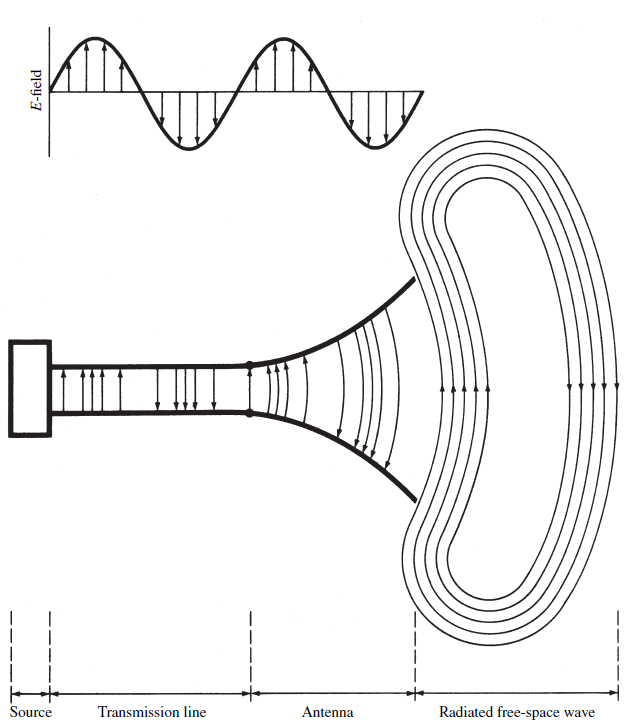
\includegraphics[scale=0.6]{chapters/ch3/assets/Antenna_transicao}
\decoRule
\caption[antena transicao]{Antena como um meio de transição (Figura 1.1 - \cite{Balanis2016})}
\label{fig:antena transicao}
\end{figure}

\subsection{Tipos de Antenas}
Neste subcapítulo irá ser introduzido de uma forma breve, os vário tipos de antenas, a sua utilização e vantagens entre estes. 

\subsection*{Antenas de Fio}
Estas antenas são umas das mais antigas, que apresentam uma configuração mais simples, sendo apenas constituídas por um fio que pode variar na sua dimensão e na sua forma e ainda podem ser utilizadas nas mais variadas aplicações. Podem tomar uma forma aleatória, desde um fio direito (dipolo) até um fio com as mais diversas formas. \par 
As antenas de fio podem ser encontradas nos mais variados locais, desde aeronaves, carros ou navios a edifícios. \par 


\subsection*{Antenas de Abertura}

\subsection*{Antenas Microstrip}

\subsection*{Antenas de Matrizes}

\subsection*{Antenas de Lente}

\subsection*{Antenas Refletora}



\section{Simulação de uma Antena}


\subsection{Para Sinais DVB-T}

